
\let\negmedspace\undefined
\let\negthickspace\undefined
\documentclass[journal]{IEEEtran}
\usepackage[a5paper, margin=10mm, onecolumn]{geometry}
%\usepackage{lmodern} % Ensure lmodern is loaded for pdflatex
\usepackage{tfrupee} % Include tfrupee package

\setlength{\headheight}{1cm} % Set the height of the header box
\setlength{\headsep}{0mm}     % Set the distance between the header box and the top of the text

\usepackage{gvv-book}
\usepackage{gvv}
\usepackage{cite}
\usepackage{amsmath,amssymb,amsfonts,amsthm}
\usepackage{algorithmic}
\usepackage{graphicx}
\usepackage{textcomp}
\usepackage{xcolor}
\usepackage{txfonts}
\usepackage{listings}
\usepackage{enumitem}
\usepackage{mathtools}
\usepackage{gensymb}
\usepackage{comment}
\usepackage[breaklinks=true]{hyperref}
\usepackage{tkz-euclide} 
\usepackage{listings}
% \usepackage{gvv}                                        
\def\inputGnumericTable{}                                 
\usepackage[latin1]{inputenc}                                
\usepackage{color}                                            
\usepackage{array}                                            
\usepackage{longtable}                                       
\usepackage{calc}                                             
\usepackage{multirow}                                         
\usepackage{hhline}                                           
\usepackage{ifthen}                                           
\usepackage{lscape}
\begin{document}

\bibliographystyle{IEEEtran}
\vspace{3cm}
\title{1.4.9.d}
\author{EE24BTECH11025 - GEEDI HARSHA}
% \maketitle
% \newpage
{\let\newpage\relax\maketitle}

\renewcommand{\thefigure}{\theenumi}
\renewcommand{\thetable}{\theenumi}
\setlength{\intextsep}{10pt} % Space between text and floats


\numberwithin{equation}{enumi}
\numberwithin{figure}{enumi}
\renewcommand{\thetable}{\theenumi}

\textbf{Question:}Given that $\vec{P}(3,2,-4)$ , $\vec{Q}(5,4,-6)$ and $\vec{R}(9,8,-10)$ are collinear. Find the ratio in which Q divides PR.\\
\begin{table}[h!]    
  			\centering
  			\begin{tabular}[12pt]{|c|c|c|c|c|c|c|c|}
\hline
Option & Anuj & Bhola & Chandan & Dilip & Eswar & Faisal \\
\hline
(A) & 6 & 2 & 5 & 1 & 3 & 4 \\
\hline
(B) & 2 & 6 & 5 & 1 & 3 & 4 \\
\hline
(C) & 4 & 2 & 6 & 3 & 1 & 5 \\
\hline
(D) & 2 & 4 & 6 & 1 & 3 & 5 \\
\hline
\end{tabular}

  			\caption{Input Parameters}
  			\label{tab1.4.9.d}
		\end{table}

	

 
		\solution As $Q$ lies between $P$ and $R$, $P$ can be represented as\\ 
		\begin{align}
			Q &=\frac{kR+P}{k+1}
		\end{align}	
			where k is the ratio,\\
		\begin{align}
			Q &=\frac{k\myvec{9\\8\\-10}+\myvec{3\\2\\-4}}{k+1} \\
			Q &=\frac{\myvec{9k+3\\8k+2\\-10k-4}}{k+1} \\
			Q &=\myvec{5\\4\\-6}
		\end{align}
			on equating both sides \\
		\begin{align}
			k=\frac{1}{2}
                \end{align}		

		\begin{figure}
    \centering
    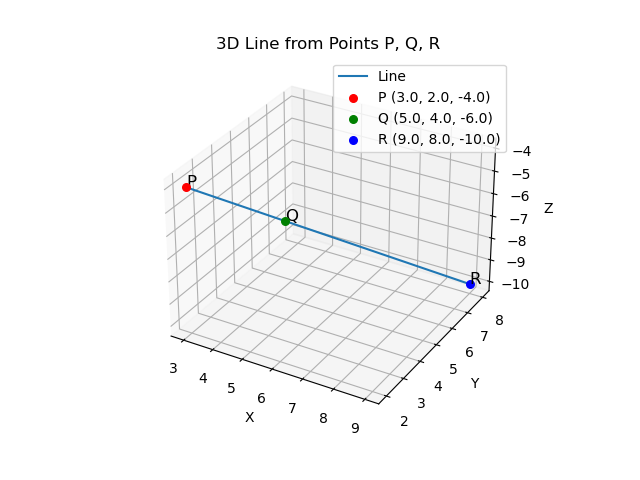
\includegraphics[width=\linewidth]{figs/fig.png}
    \caption{The Plot of the given points}
    \label{fig:your_label}
		\end{figure}
\end{document}

